\documentclass{article} 
\usepackage[utf8]{inputenc}
\usepackage{graphicx}
\usepackage{enumitem}
\graphicspath{./}
\usepackage{mathtools, amssymb, amsthm} % imports amsmath

\newcommand{\prefacename}{Preface}
\newenvironment{preface}{
    \vspace*{\stretch{2}}
    {\noindent \bfseries \Huge \prefacename}
    \begin{center}
        % \phantomsection \addcontentsline{toc}{chapter}{\prefacename} % enable this if you want to put the preface in the table of contents
        \thispagestyle{plain}
    \end{center}%
}
{\vspace*{\stretch{5}}}



\author{Daniel Palma}
\date{\today}
\title{Test 2 Review}

\begin{document}

\maketitle
\newpage

\begin{preface}
    I'm writing this in order for me not to fail this fucking Test.
    Best of luck to everyone. If I make a mistake please contact me on discord (user: \verb|dnwmn|) and I appreciate any feedback on these. I'm using the James Stewart Calculus 8th edition for my theory just so you guys know 
\end{preface}

\tableofcontents
\newpage



\section*{Topics}

\begin{itemize}
    \item Partial Derivatives
    \item Tangent Planes and Linear Approximations
    \item Chain Rule
    \item Directional Derivatives and the Gradient Vector
    \item Shapes of Functions
    \item Maximum and Minimum Values
    \item Double Integrals over Rectangles
    \item Double Integrals over General Regions
    \item How to Graph Regions when Taking Integrals
\end{itemize}


\newpage
\section*{Theory}

\section{Partial Derivatives}

In general, if $f$ is a function of two variables $x$ and $y$ supposed we take a derivative of $x$ while keeping $y$ constant, this is considered to be a partial derivative of $f$ with respect to $x$.

The same applies to y, this section is pretty straight forward it's just derivatives and keep the rest of the stuff constant.

Notation:

$$f_x(x,y) = f_x = \frac{\partial f}{\partial x} = \frac{\partial}{\partial x}f(x,y) = f_1 = D_1f = D_xf$$

$$f_y(x,y) = f_y = \frac{\partial f}{\partial y} = \frac{\partial}{\partial y}f(x,y) = f_1 = D_1f = D_yf$$

To compute partial derivatives all we have to do is remember that a partial derivative with respect to $x$ is just the normal derivative of $f$ with respect to $x$ while keeping $y$ constant.

\subsection{Interpretation}

Sure, but what does this all mean?

if $z = f(x,y)$, $f_x$ represents the rate of change of $z$ with respect to $x$ when $y$ is fixed (and vice versa) 

\subsection{Examples}

$$f(x,y) = x^3 + x^2y^3 -2y^2$$


$$f_x = 3x^3 + 2xy^3$$
$$f_y = 3x^2y^2 - 4y$$

\subsection{Higher Derivatives}

Just do it again, but now we can point out that the order of the derivatives does not matter due to claireauts theorem

\textbf{Claireauts theorem only applies if functions are continuous}

$$f_{xy} = f_{yx}$$

\newpage
\section{Tangent Planes and Linear Approximations}


\subsection{Tangent Planes}
We know that any plane passing through the point $P(x_0,y_0,z_0)$ has an equation of the form 

$$A(x-_0) + B(y-y_0) + C(z-z_0) = 0$$

by dividing this by $C$ and letting $a= \frac{-A}{C}$ and $b = \frac{-B}{C}$ we can write it in the following form

$$z - z_0 = a(x-x_0) + b(y - y_0)$$

blah blah algebra basically $z - z_0 = a(x-x_0)$ is the equation of point slope of a line of slope $a$, and we know the slope of a tangent is $f_x$ so we can say $a = f_x(x_0,y_0)$, this way we can simplify the formula to the following

$$z - z_0 = f_x \big\rvert_{(x_0,y_0)}(x-x_0) + f_y \big\rvert_{(x_0, y_0)}(y-y_0)$$

where $f_x \big\rvert_{(x_0,y_0)}$ is just $f_x$ with $(x_0, y_0)$ plugged in (applies to the rest as well)


\subsection{Linear Approximations}

In general, we know that an equation of the tangent plane to the graph of a function $f$ of two variables at the point $(a,b,f(a,b))$ is 

$$z = f(a,b) + f_x\big\rvert_{(a,b)}(x-a) + f_y\big\rvert_{(a,b)}(y-b)$$

The linear function whose graph is this tangent plane, namely

$$L(x,y) = f(a,b) + f_x\big\rvert_{(a,b)}(x-a) + f_y\big\rvert_{(a,b)}(y-b)$$

is called the linearization of $f$ at $(a,b)$ and the approximation

$$f(x,y) \approx f(a,b) + f_x\big\rvert_{(a,b)}(x-a) + f_y\big\rvert_{(a,b)}(y-b)$$

is called the linear approximation or the tangent plane approximation of $f$ at $(a,b)$


\subsection{Total Differential}

$$dz = \frac{\partial z}{\partial x}dx + \frac{\partial z}{\partial y}dy $$

way easier to calculate this versus the increment lmfao 


\subsection{Three or more variables}

same conventions as before nothing too crazy

\newpage
\section{Chain Rule}

Recall that the chain rule for functions of a single variable gives the rule for differentiating a composite function, if $y = f(x)$ and $x = g(t)$ where $f$ and $g$ are dfferentiable functions, then y is indirectly a function of $t$ and can be written as 

$$\frac{dy}{dt} = \frac{dy}{dx} \times \frac{dx}{dt} $$

the easiest way to do this is to draw a dependency tree, and then follow the following rules:

\begin{itemize}
    \item Draw a dependency tree with each function as a node and then each child of this m-way tree is the corresponding parameters of that function
    \item for each factor $m$ there will be $n$ terms determined by doing an inorder search for variable $t$ that is where $t$ is the term being differentiated with respect to and $n$ is the depth of the target node
    \item each appearance of the node $t$ will correspond directly to the amount of factor $m$ in the resulting formula.
\end{itemize}

Example: if $z = f(x,y)$ and $x = g(s,t)$ and $y = h(s,t)$ then we can draw a dependency tree as follows to find $\frac{\partial z}{\partial s}$

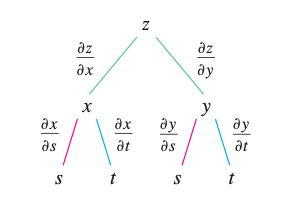
\includegraphics[scale=1]{dptree.png}

as such, following the inorder traversal we get the following formula for $\frac{\partial z}{\partial s}$

$$\frac{\partial z}{\partial s} = \frac{\partial z}{\partial x}\frac{\partial x}{\partial s} + \frac{\partial z}{\partial y} \frac{\partial y}{\partial s}$$

so we can see, we performed a search for the term $s$. $m$ is the number of factors that corresponds to the number of appearances of $s$, so in this case we have 2, and each factor has $n$ terms, in this case each factor had 2 terms since the depth of the target node $s$ in each case was 2


\newpage
\section{Directional Derivatives and the Gradient Vector}

\subsection{Directional Derivative}

If $f$ is a differentiable function of $x$ and $y$, then $f$ has a directional derivative in the direction of any unit vector $\vec{u} = \langle a,b \rangle$ and

$$D_uf(x,y) = f_x(x,y)a + f_y(x,y)b$$

this is the same as saying

$$D_uf(x,y) = \nabla f \cdot \vec{u}$$

where $\nabla f$ is 

$$\nabla f  = \langle f_x, f_y \rangle$$

If the unit vector $\vec{u}$ makes an angle $\theta$ then we can write $\vec{u} = \langle cos \theta, sin \theta \rangle$

\subsection{Gradient Vector}


Formal Definition:

$$\nabla f(x,y) = \langle f_x, f_y \rangle = \frac{\partial f}{\partial x}\hat{i}+\frac{\partial f}{\partial y} \hat{j}$$

In what direction does $f$ change the fastest and what is the maximum rate of change? the answers are provided by the following theorem:

\begin{center}
    Suppose $f$ is a differentiable fuction of two or three variables. The maximum value of the directional derivative $D_uf(\mathbf{x}) $ is $\rvert \nabla f(\mathbf{x}) \rvert$ and it occurs when $\vec{u}$ has the same direction as the gradient vector $\nabla f(\mathbf{x})$.
\end{center}

\newpage
\section{Shapes of Functions !!TODO!!}

\newpage
\section{Maximum and Minimum Values}

Theorem:
\begin{center}
    if $f$ has a local maximum or minium at $(a,b)$ and the first-order partial derivative of $f$ exist there, then $f_x(a,b) = 0$ and $f_y(a,b) = 0$.
\end{center}

A point $(a,b)$ is called a \textbf{critical point} (or stationary point i guess) of $f$ if $f_x(a,b) = 0$ and $f_y(a,b) = 0$, or if one of these partial derivatives do not exist. However, not all critical points give a maxima or minima, at a critical point, a function could have a local mximum or a local minimum or neither. (Saddle points!) 

We need a way to classify these critical points, and that's why we have the second derivative test.


$$D = f_{xx}(a,b)f_{yy}(a,b) + (f_{xy}(a,b))^2$$

we can now classify a point $(a,b)$ as follows:

\begin{itemize}
    \item If $D > 0$ and $f_{xx}(a,b) >0$ then $(a,b)$ is a local minimum
    \item If $D>0$ and $f_{xx}(a,b)<0$ then $(a,b)$ is a local maximum
    \item If $D<0$ then $(a,b)$ is a Saddle point
    \item If $D=0$ then the test is inconclusive
\end{itemize}

\subsection{Absolute Maximum and Minimum Values}

To find the absolute maximum and minimum values of a continuous function $f$ on a closed, bounded set $D$:

\begin{enumerate}
    \item Find the values of $f$ at the critical points of $f$ in $D$.
    \item Find the extreme values of $f$ on the boundary of $D$.
    \item The largest of the values from steps 1 and 2 is the absolute maximum value; the smallest is the absolute minimum value.
\end{enumerate}

I'm gonna be honest i dont really fucking know how to do this one we ball

\newpage
\section{Double Integrals over Rectangles}

The \textbf{double integral} of $f$ over the rectangle $R$ is
$$\iint\limits_{R}f(x,y)\mathrm{d}A = \lim_{m,n \rightarrow \infty}\sum_{i=1}^{m}\sum_{j=1}^{n}f(x_{ij}^*, y_{ij}^*)\Delta A$$

if this limit exists.

Thus, if $f(x,y) \geq 0$, then the volume $V$ of the solid that lies above the rectangle $R$ and below the surface $z = f(x,y)$ is 

$$V = \iint\limits_{R}f(x,y)\mathrm{d}A$$

\subsection{Iterated Integrals}

this is just the nicer way of doing shit tbh

either of the following

$$\int^b_a\int^d_cf(x,y)dy dx$$

$$\int^d_c\int^b_af(x,y)dxdy$$

so whichever one on the inside that's the respective partial integration

in the first one, we would integrate with respect to y first and then x, and vice versa in the second one.

Iterated Integrals are much nicer so we have "Fubini" to thank for his amazing theorem 

If $f$ is continuous on the rectangle blah blah (this is fubinis theorem)

$$\iint\limits_{R}f(x,y)\mathrm{d}A = \int^b_a\int^d_cf(x,y)dy dx  = \int^d_c\int^b_af(x,y)dxdy$$


\subsection{Average Value}

 We define the \textbf{average value} of a function $f$ of two variables defined on a rectangle $R$ to be

$$f_{ave} = \frac{1}{A(R)}\iint\limits_{R}f(x,y)\mathrm{d}A$$

Where $A(R)$ is the area of R


\newpage
\section{Double Integrals over General Regions}

(domains i guess)

We can suppose $D$ is a bounded region, we can say that if $F$ is integrable over $R$ ( a rectangle formed around $D$ ) we can define the \textbf{double integral of $f$ over $D$} by 

$$\iint\limits_{D}f(x,y)\mathrm{d}A = \iint\limits_{R}F(x,y)\mathrm{d}A$$

\subsubsection*{Type 1 Regions}

A plane region $D$ is said to be of \textbf{type I} if it lies between the graphs of two continuous functions of x (y = a function of x)

and can be given the following formula

$$\iint\limits_{D}f(x,y)\mathrm{d}A = \int^b_a\int^{g_2(x)}_{g_1(x)} f(x,y) dy dx$$

\subsubsection*{Type 2 Regions}

A plane region $D$ is said to be of \textbf{type II} if it lies between the graphs of two continuous functions of y (x = a function of y)

and can be given the following formula

$$\iint\limits_{D}f(x,y)\mathrm{d}A = \int^d_c\int^{h_2(y)}_{h_1(y)} f(x,y) dx dy$$

\subsection{Properties of Double Integrals}

We assume that all of the following integrals exist.

\begin{enumerate}
    \item $\iint\limits_{D}[f(x,y) + g(x,y)]\mathrm{d}A = \iint\limits_{D}f(x,y)\mathrm{d}A + \iint\limits_{D}g(x,y)\mathrm{d}A$
    \item $\iint\limits_{D}cf(x,y)\mathrm{d}A = c \iint\limits_{D}f(x,y)\mathrm{d}A$
\end{enumerate}

If $f(x,y) \geq g(x,y)$ for all $(x,y)$ in $D$

\begin{enumerate}
    \item $\iint\limits_{D} f(x,y) \mathrm{d}a \geq \iint\limits_{D}g(x,y) \mathrm{d}A$
\end{enumerate}

The next property is the same as when you split an integrals region from $a \rightarrow b  = a \rightarrow c + c \rightarrow b$

$$\iint\limits_{D}f(x,y)\mathrm{d}A = \iint\limits_{D_1}f(x,y)\mathrm{d}A + \iint\limits_{D_2}f(x,y)\mathrm{d}A$$

where $D = D_1 \cup D_2 $,$D_1$ and $D_2$ dont overlap except perhaps on their boundaries

This property is especially useful when a region does not classify as either Type I nor Type II but can be expressed as a union of regions of type I or type II

This next property of integrals says that if we integrate the constant function $f(x,y) = 1$ over a region $D$ we get the area of $D$:

$$\iint\limits_{D}1\mathrm{d}A = A(D)$$

\newpage
\section{How to Graph Regions when Taking Integrals !!TODO!!}

\section{Triple Integrals (short section)}

    Find the total amount of $f(x,y,z)$ on $E$

    Definition of the triple integral

    $$\iiint\limits_{E}f(x,y,z)\mathrm{d}V$$

    \subsection{Type I 3D region}

    \subsection{Type II 3D region}

    \subsection{Type III 3D region}

\newpage
\section{Review Sheet Problems and Solutions}

\newpage
\section{Formula Sheet}

\end{document}